\section{CouchDB}
\subsection{Cluster Setup}
 From CouchDB documentation (CITE THIS), cluster of 3 nodes work well, 8 shards 2 replicas 

\subsection{Database} 
After installation and initial start-up of three nodes in the cluster, we need to make sure three nodes can be joined with each other before creating databases. 

At first, we planned to create one database includes all of tweets from harvester. Then we created a design document and select text as a index of query. Because there are three scenarios about the attitudes to covid19, covidsafe app and the popular symptoms of covid19 in different area of Australia, it was better to analyze that separating all of tweets into one partition database including 4 partition keys according to full-text search method. 

\begin{figure}[H]
    \centering
    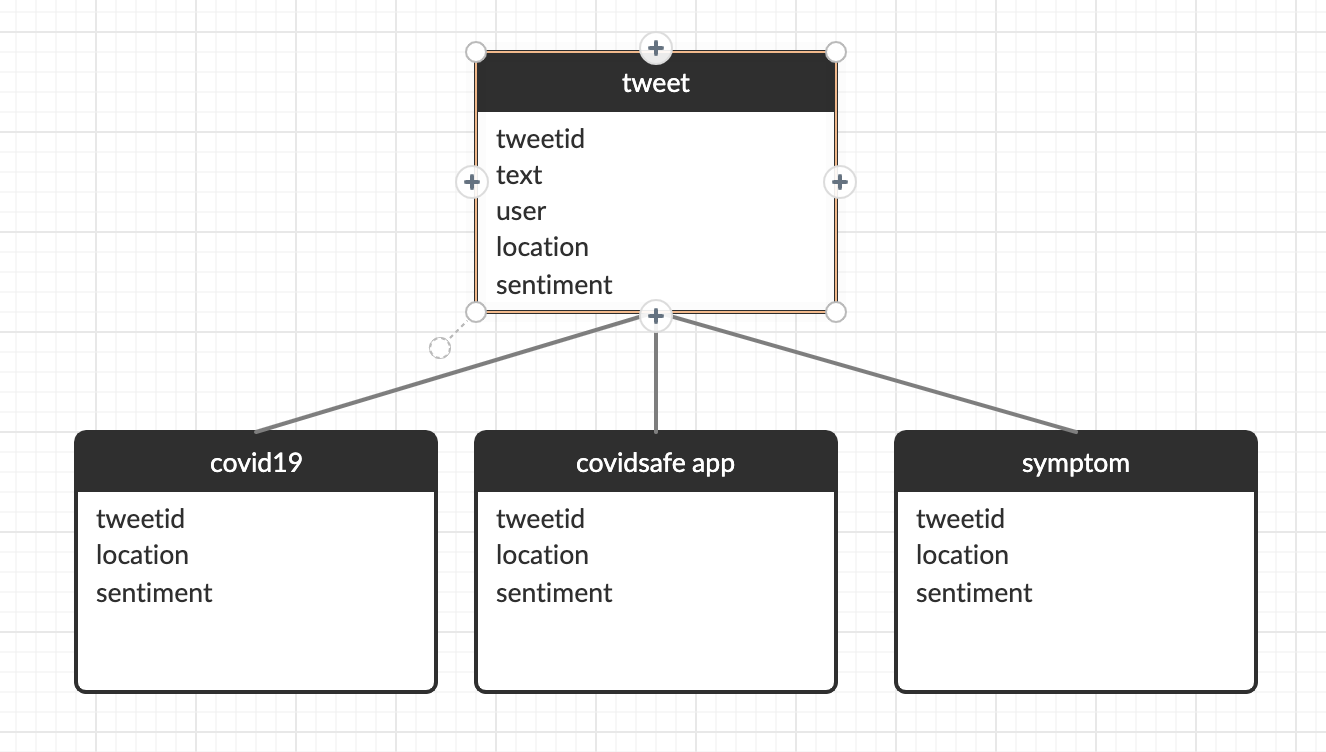
\includegraphics[scale=0.4]{city_analytics/report/images/db1.png}
    \caption{Original design database}
    \label{fig:my_label}
\end{figure}

But the one of biggest challenges from this method was the size of data.  If we handle with all tweets in a 6GB database, it would spend a lot of time waiting the results of query. Thus, it's too slow to be usable to update the results. Because when the new documents are coming, couchDB will query all documents again.

Therefor, we tried to filter tweets locally for the purpose of analysis and threw away tweets those are not related to our scenarios. After harvesting all tweets, we determined if this tweet is relevant to our topics. We created three partition couchdbs with 8 shards and 2 replicas and loaded relevant data into database. Different topics are stored in different partition databases.

\begin{figure}[H]
    \centering
    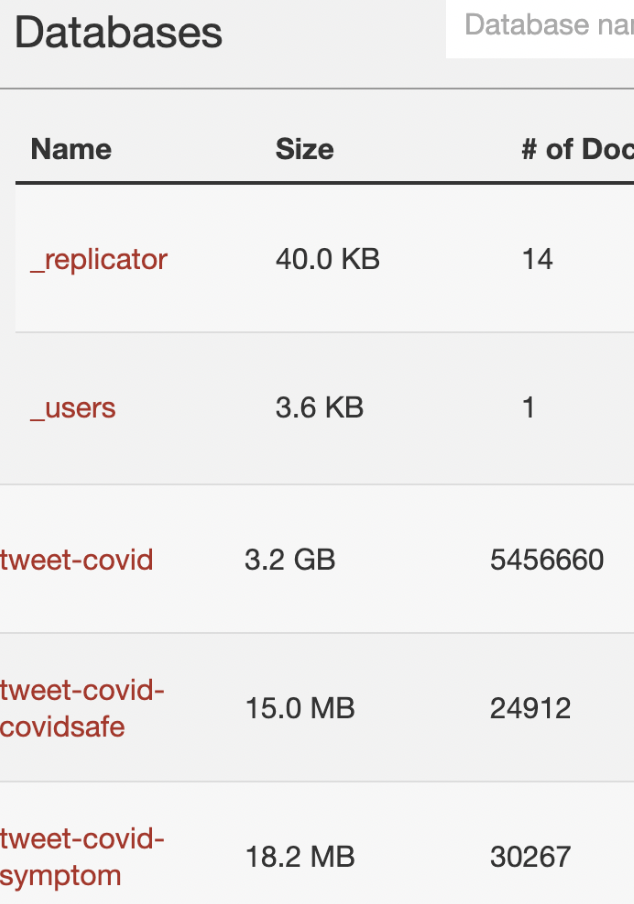
\includegraphics[scale=0.4]{city_analytics/report/images/couchdb.png}
    \caption{couchDB}
    \label{fig:my_label}
\end{figure}

For each database, it has three partition keys according to SA4 source.It's convenient for us to select different key. When we want to draw the points into map, we can set the partition key is 'geo' to get the coordinates of tweets. The time of creating view in a partition database is less than that in a non-partition database because database doesn't need to scan all the documents. 

\begin{figure}[H]
    \centering
    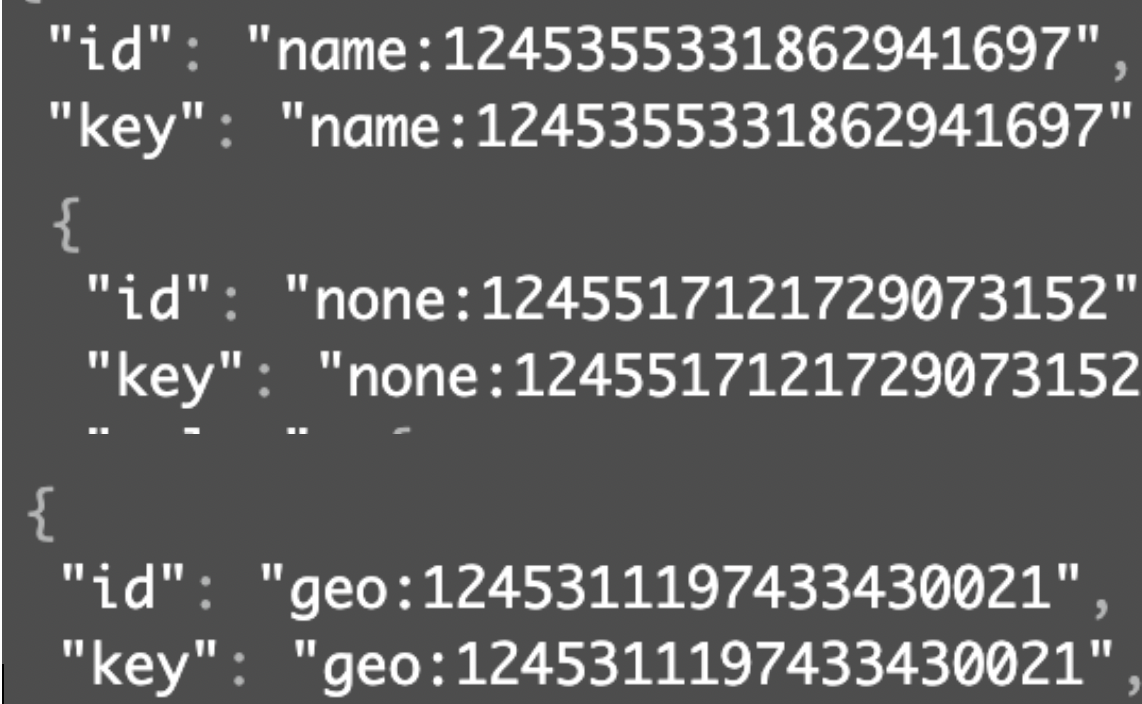
\includegraphics[scale=0.4]{city_analytics/report/images/partitionkey.png}
    \caption{Partition key in one couchDB}
    \label{fig:my_label}
\end{figure}

For the tweet-covid-symptom couchDB, the goal of our topics is to check the nunmber of tweets including the covid symptoms and show which symptoms are more common in Australia. So we selected ten symptoms and they were fever, cough, sore throat, breathing, body-ache, diarrhoea, fatigue, headache, vomit and loss of sense of smell. We used query function and made a selector to select which symptom the tweets contains. What's more, all of tweets in the 'tweet-covid-symptom' would get a new entity 'symptoms' that including the symptoms contained in that tweet and be loaded in a new couchDB name 'symptoms'. In this new couchDB, the documents only includes SA4, timestamp,symptoms and sentiment entity.

\begin{figure}[H]
    \centering
    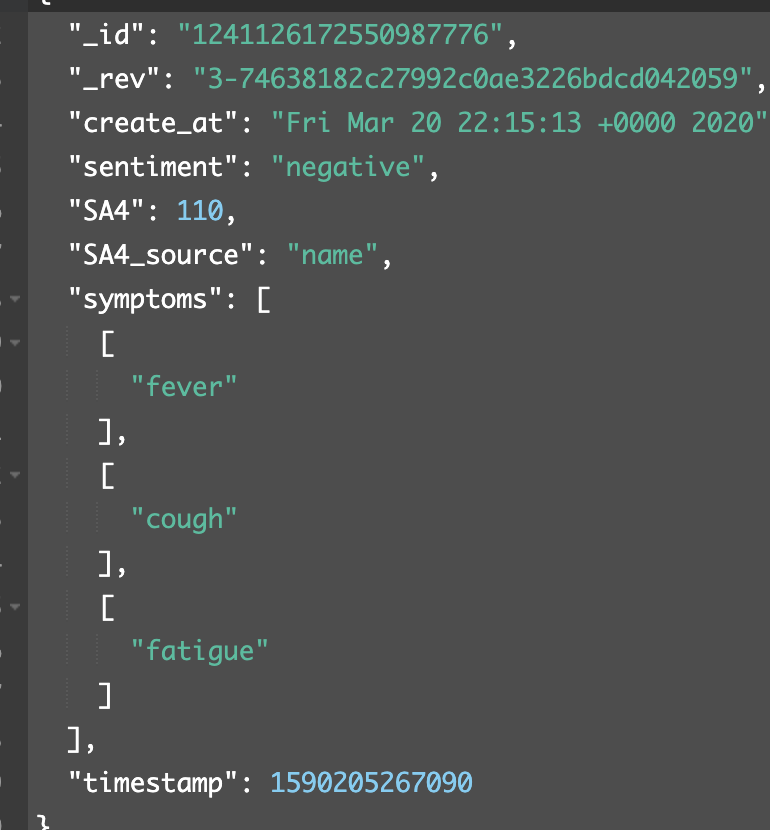
\includegraphics[scale=0.4]{city_analytics/report/images/symptomsdb.png}
    \caption{one document in symptoms}
    \label{fig:my_label}
\end{figure}

To reduce the query time and update graph in page faster, the view about timestamp was created in 'symptoms' database. This view would collect the max timestamp number when we query the view and we updated view in every 15 seconds. During querying in 'tweet-covid-symptom', the selector would choose the timestamp was greater than the max one in the 'symptoms' and check which symptom that tweet contained. 

\subsection{View initialization}

To make the server run more smoothly and stable, we used python-cloudant to access couchDB. Design documents and views were directly created in the python file. So we created one mapreduce function in each database. In 'tweet-covid', and 'tweet-covid-covidsafe', we selected sentiment and SA4 as key and counted the number of tweet in same sentiment and same area. In 'symptoms', symptom, SA4 source and SA4 was treated as key and do the same reduce function as other databases. 

\begin{figure}[H]
    \centering
    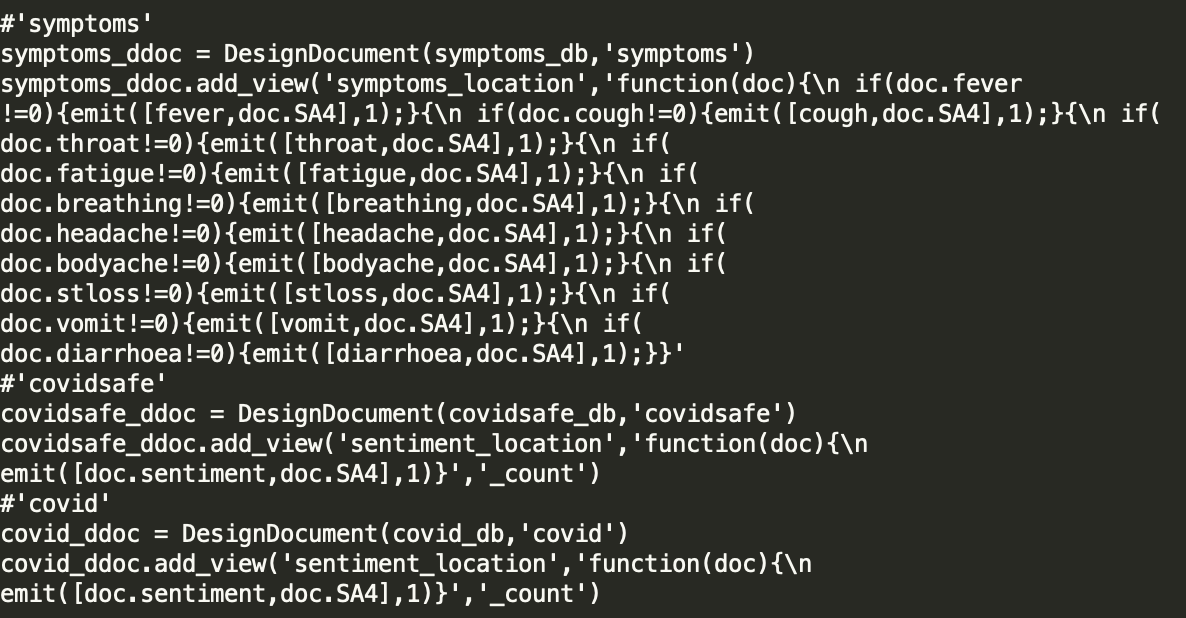
\includegraphics[scale=0.5]{city_analytics/report/images/view.png}
    \caption{views code in python file}
    \label{fig:my_label}
\end{figure}

After creating views, 